% Chapter 3

\chapter{Solution n° 2} % Main chapter title

\label{Chapter3} % For referencing the chapter elsewhere, use \ref{Chapter3}
%----------------------------------------------------------------------------------------
\begin{description}
  \item[Version du Kernel :] 4.14
\end{description}

\section{Kernel 4.14}
La version 4.14 (une des plus recente chez fslc) du kernel contient un driver imx219
main line operationel. Notre idée était de porter le suport de la meta-voipac compatible
avec un kernel 4.1 sur le nouveau kernel 4.14 pour pouvoir utiliser le driver.

\section{Travail effectué}
\textbf{Modifier les sources du Kernel}

 Dans les recettes kernel chaque version du kernel est architecturé de la meme façon :
  \begin{itemize}
  \item[-] Créer un fichier linux-voipac\_4.14.bb.
  \item[-] Créer un document linux-voipac-4.14 content un defconfig et un patch du device tree Openrex.
  \end{itemize}

\begin{figure}[th]
  \centering
  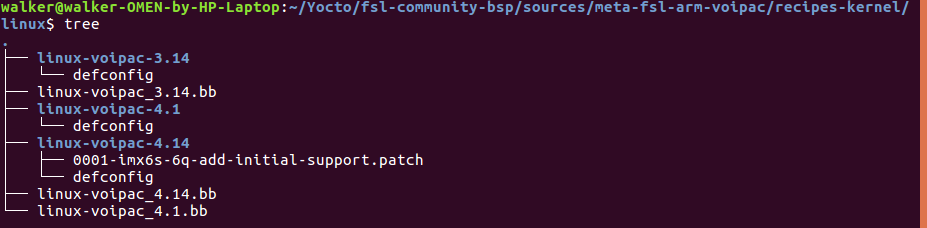
\includegraphics[width=1\linewidth]{tre.png}
  \decoRule
  \caption{arborescence des fichiers}  \label{fig:planning}
\end{figure}

Le principe de cette méthode et de copier la version 4.1 et de remplacer les sources du kernel. 

\begin{description}
  \item[Modification du fichier]
    \begin{lstlisting}
      SRCBRANCH = "4.14.x+fslc"
      LOCALVERSION = "-yocto"
      SRCREV = "${AUTOREV}"
      KERNEL_SRC ?= "git://github.com/Freescale/linux-fslc.git;protocol=git"
    \end{lstlisting}
\end{description}

\section{Erreur}

\begin{figure}[th]
  \centering
  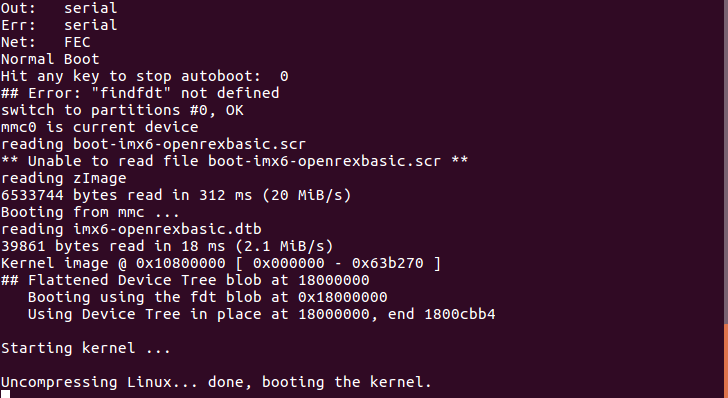
\includegraphics[width=1\linewidth]{4-14boot.png}
  \decoRule
  \caption{phase de boot}  \label{fig:planning}
\end{figure}

\section{Conclusion}


%----------------------------------------------------------------------------------------
